\section{Theorie}
\label{sec:Theorie}

Das Geiger-Müller-Zählrohr wird verwendet, um die Intensität ionisierender Strahlung 
zu messen. Dabei werden elektrische Impulse erzeugt, wenn $\alpha$-, $\beta$- oder
$\gamma$- Teilchen absorbiert werden. Im vorliegenden Versuch sollen einige Kenndaten 
eines solchen Zählrohrs experimentell bestimmt werden. 

\subsection{Aufbau und Charakteristik}

Der schematische Aufbau ist in Abbildung \ref{fig:aufbau} zu erkennen. 

\begin{figure}
  \centering
  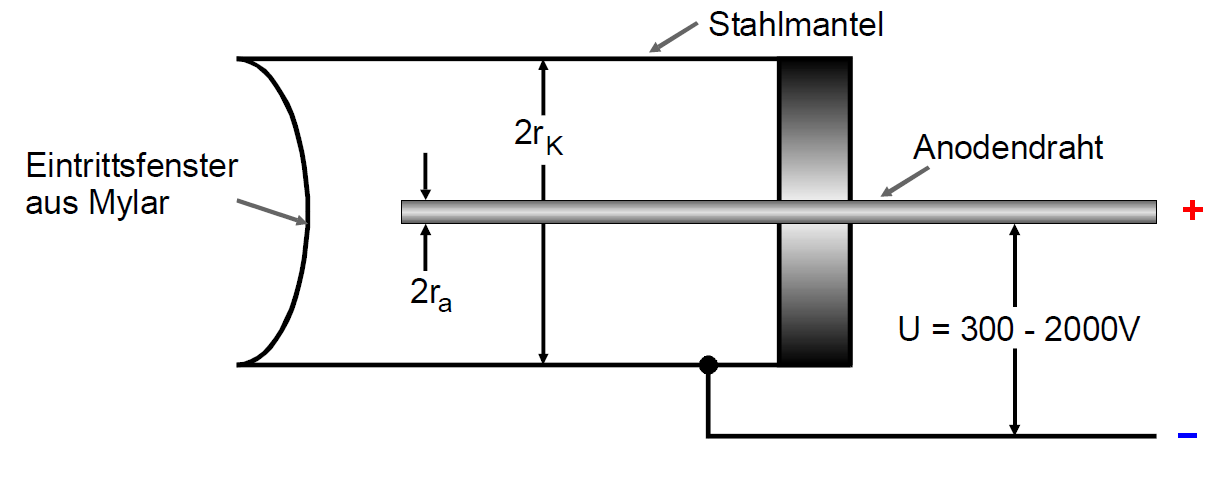
\includegraphics[scale=0.4]{content/Querschnitt.png}
  \caption{Querschnitt eines Endfenster-Zählrohrs [1]}
  \label{fig:aufbau}
\end{figure}

Das Geiger-Müller-Zählrohr besteht aus einem Kathodenzylinder und einem darin axial
verlaufendem Anodendraht. Im Inneren befindet sich ein Gasgemisch. Das Anlegen einer
Spannung führt zu einem radialsymmetrischen Feld zwischen Kathode und Anode. 
Wenn ein geladenes Teilchen in das Zählrohrvolumen eindringt und vollständig 
absorbiert wird, werden durch Ionisationsakte freie Elektronen und Ionen erzeugt. 
Die Anzahl der entstehenden Elektronen ist dabei proportional zur Energie des 
einfallenden Teilchens. In Abbildung \ref{fig:Elektronen} ist erkennbar, dass die Zahl der erzeugten
Elektronen von der Zählrohrspannung $U$ abhängt. Es ist möglich, dass diese nicht 
ausreicht, damit alle Elektronen den Draht erreichen, da viele durch Rekombination 
verloren gehen (Bereich I). 

\begin{figure}
  \centering
  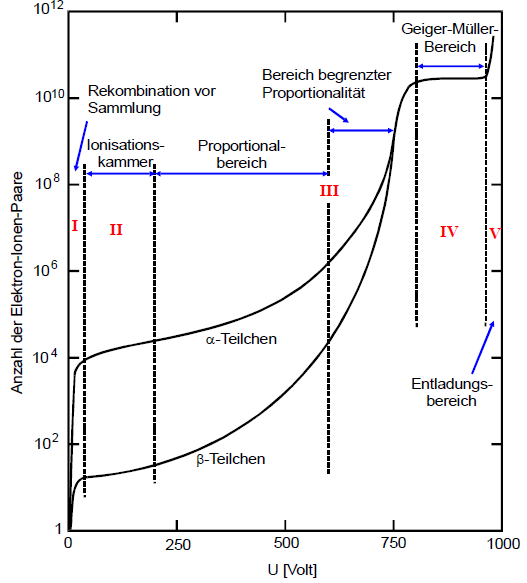
\includegraphics[scale=0.6]{content/Bereiche.pg.png}
  \caption{Detektierte Elektronen in Abhängigkeit von der Zählrohrspannung [1]}
  \label{fig:Elektronen}
\end{figure}

Der Ionisationsstrom ist bei ausreichender Spannung proportional zur Energie 
der einfallenden Strahlung. Diesen Bereich bezeichnet man als Ionisationskammer
(Bereich II). Durch die geringen Ströme, kann diese Kammer praktisch nur für hohe 
Strahlintensität eingesetzt werden. 

Daran schließt sich der Proportionalitätsbereich (Bereich III) an. In diesem haben
die Elektronen eine Energie, die hoch genug ist, durch Stoßionisation ihrerseits
ionisieren zu können. Die dadurch erzeugten freien Elektronen können ebenfalls
ionisieren. Wegen des Anstiegs der Anzahl der freien Elektronen wird dieser Prozess
als Townsend-Lawine bezeichnet. Die gesammelte Ladung $Q$ ist proportional zur
Primärteilchenenergie, sodass das Proportionalzählrohr zur Energiemessung der 
einfallenden Strahlung geeignet ist. 

Eine noch höhere Spannung führt zu dem Auslösebereich (Bereich IV). Die Ladung Q 
ist in diesem Bereich unabhängig von der Primärionisation, sondern hängt nur noch
vom Volumen und der Spannung ab. Durch die Entstehung von ungeladenen UV-Photonen, 
die sich senkrecht zum E-Feld ausbreiten können, werden so weitere Lawinen im 
gesamten Zählrohrvolumen ausgelöst. Das Geiger-Müller-Zählrohr kann nur noch für
Intensitätsmessung benutzt werden. Der lineare Teil in diesem Bereich wird als
Plateau bezeichnet. 
Die Kenndaten eines Zählrohrs sind die Länge des Plateaus und dessen Anstieg. Je
niedriger die Steigung und je länger das Plateau ist, desto hochwertiger ist das
Geiger-Müller-Zählrohr. 

Wenn die Spannung $U$ noch weiter erhöht wird, wird durch ein einzelnes Teilchen 
die Dauerentladung gezündet. Dies zerstört schnell das Zählrohr (Bereich V). 

\subsection{Totzeit und Nachentladung}

Nach einer Entladung verbleiben Ionen wegen ihrer größeren Masse länger als 
die Elektronen im Gasraum und bauen einen sogenannten Ionenschlauch auf. 
Danach ist für eine Zeit $T_\text{T}$ keine Stoßionisation möglich, da die 
effektive Feldstärke in Drahtnähe reduziert wird. In diesem Zeitraum können 
keine weiteren Teilchen detektiert werden. Deswegen wird $T_\text{T}$ als 
Totzeit des Zählrohres bezeichnet. Zudem kann der Ladungsimpuls seine 
ursprüngliche Höhe erst nach vollständiger Neutralisation der Ionen erreichen. 
Daher schließt sich an die Totzeit die längere Erholungszeit $T_\text{E}$ 
an. Diese Zeiträume sind in Abbildung \ref{fig:Totzeit} dargestellt. 

\begin{figure}
  \centering
  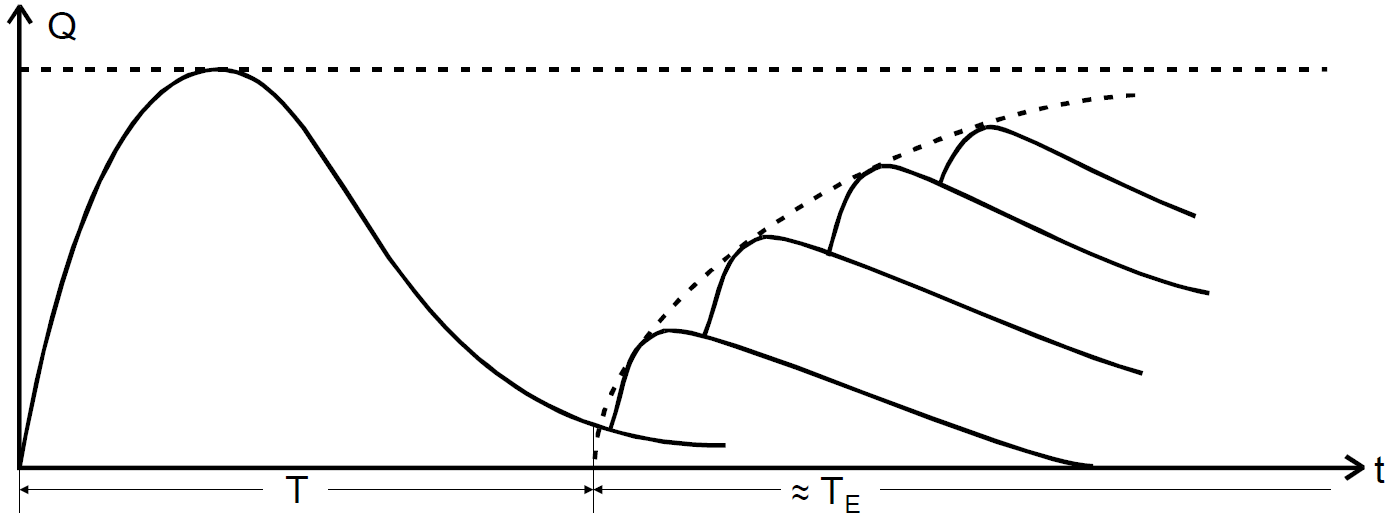
\includegraphics[scale=0.3]{content/Totzeit.png}
  \caption{Qualitative Darstellung der Tot- und Erholungszeit eines Zählrohrs [1]}
  \label{fig:Totzeit}
\end{figure}

Mit einem Oszilloskop ist es möglich, diese Kurve sichtbar zu machen, sodass die
Totzeit $T_\text{T}$ direkt abgelesen werden kann. Außerdem kann zur Bestimmung 
der Totzeit auch die in Kapitel 2 erläuterte Zwei-Quellen-Methode verwendet werden. 
Die Totzeit berechnet sich nach 

\begin{equation}
T_\text{T} \approx \frac{n_1+n_2-n_\text{1+2}}{2n_1n_2}.
\label{eqn:totzeit}
\end{equation}

Die $n_\text{i}$ sind dabei die Impulsraten.

Sogenannte Nachentladungen können während der Erholungszeit stattfinden. Diese 
enstehen dadurch, dass Ionen beim Neutralisieren am Zählrohrmantel Elektronen 
herauslösen, welche wiederum neue Elektronenlawinen auslösen. Zum Reduzieren 
dieser Nachentladung wird dem Gas ein Alkoholzusatz beigemischt, welcher die 
Ionen im Gasraum neutralisiert. Die positiv geladenen Alkoholmoleküle wandern
dann anstatt der Ionen zum Zählrohrmantel und werden dort neutralisiert, ohne 
weitere Elektronenlawinen auszulösen. 